\section{第1章\quad 绪论}

\begin{frame}{近代通信技术的发展}
 \begin{columns}
  \begin{column}{0.35\linewidth}
   \centering
   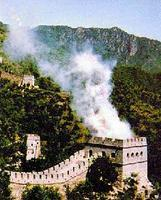
\includegraphics[height=5cm]{fenghuotai2.jpg}
  \end{column}
  \begin{column}{0.65\linewidth}
   \centering
   \begin{itemize}
    \item 人类历史上最早的通信手段和现在一样是“无线”的。
    \item 人类通信史上革命性变化,是从把电作为信息载体后发生的。
   \end{itemize}
  \end{column}
 \end{columns}
\end{frame}

\begin{frame}{电报的发明}
 \begin{columns}
  \begin{column}{0.5\linewidth}
   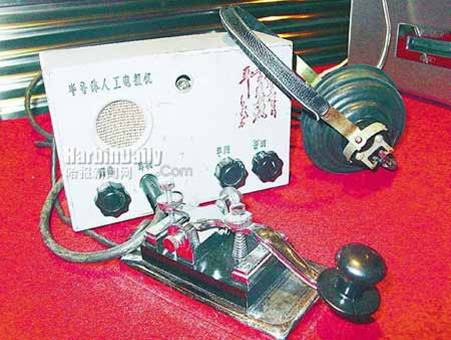
\includegraphics[height=4cm]{dianbao}
  \end{column}
  \begin{column}{0.5\linewidth}
   \begin{itemize}
    \item 电报的发明,拉开了电信时代的序幕,开创了人类利用电来传递信息的历史。
   \end{itemize}
  \end{column}
 \end{columns}
\end{frame}

\begin{frame}{电报的发明}
 \begin{columns}
  \begin{column}{0.5\linewidth}
   \begin{figure}
    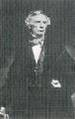
\includegraphics[width=3.5cm]{Morse.jpeg}
    \caption{莫尔斯 Morse.Samrel Finley.Breese (1791-1872)}\label{Morse}
   \end{figure}
  \end{column}
  \begin{column}{0.5\linewidth}
   \begin{itemize}
    \item 美国画家莫尔斯
    \item 在1835年,第一台电报机问世
   \end{itemize}
  \end{column}
 \end{columns}
\end{frame}

\begin{frame}{电报的发明}
 \begin{itemize}
  \item 莫尔斯成功地利用电流的“通”、“断”和“长断”来代替了人类的文字进行传送,这就是鼎鼎大名的莫尔斯电码。
 \end{itemize}
 \centering
 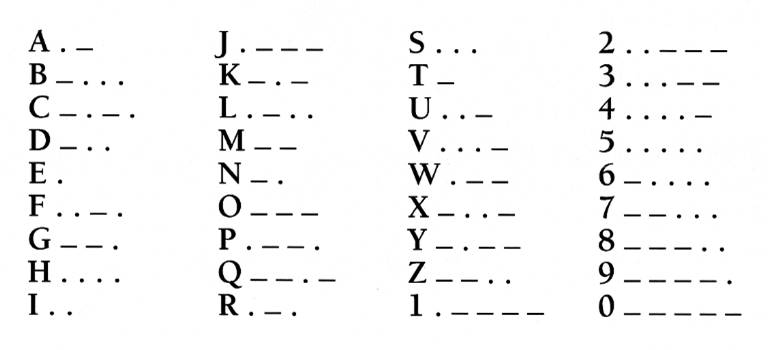
\includegraphics[width=8cm]{morsecode}
\end{frame}

\begin{frame}{电话的发明}
 \begin{columns}
  \begin{column}{0.35\linewidth}
   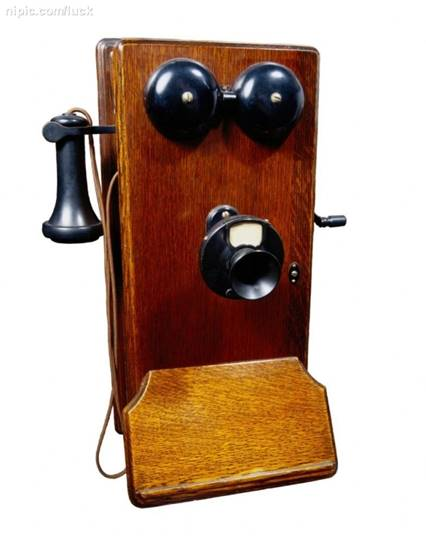
\includegraphics[height=6.5cm]{dianhua}
  \end{column}
  \begin{column}{0.65\linewidth}
   \begin{itemize}
    \item 1875年6月2日,被人们作为发明电话的伟大日子而加以纪念,而美国波士顿法院路109号也因此载入史册,至今它的门口仍钉着块铜牌,上面镌有:“1875年6月2日电话诞生在此。”
   \end{itemize}
  \end{column}
 \end{columns}
\end{frame}

\begin{frame}{电话的发明}
 \begin{columns}
  \begin{column}{0.4\linewidth}
   \begin{figure}
    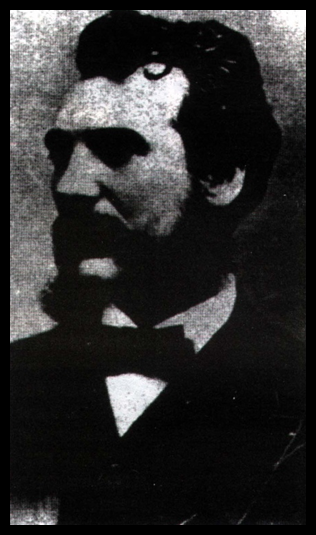
\includegraphics[width=3.5cm]{Bell.jpg}
    \caption{亚历山大·格拉汉姆·贝尔Alexander Graham Bell (1847 - 1922)}
   \end{figure}
  \end{column}
  \begin{column}{0.6\linewidth}
   \begin{itemize}
    \item 美国发明家和企业家。他获得了世界上第一台可用的电话机的专利权(发明者为意大利人安东尼奥·梅乌奇),创建了贝尔电话公司(AT\&T公司的前身)。其被世界誉为“电话之父”。
   \end{itemize}
  \end{column}
 \end{columns}
\end{frame}

\begin{frame}{电话的发明}
 \begin{columns}
  \begin{column}{0.5\linewidth}
   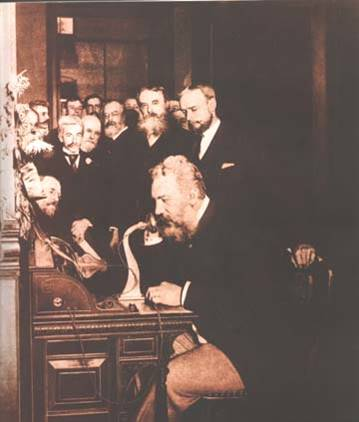
\includegraphics[width=5.5cm]{Bell2}
  \end{column}
  \begin{column}{0.5\linewidth}
   \begin{itemize}
    \item 贝尔在1892年启用第一条长途电话线——从纽约至芝加哥,长约900里。
   \end{itemize}
  \end{column}
 \end{columns}
\end{frame}

\begin{frame}{电话的发明}
 \begin{columns}
  \begin{column}{0.35\linewidth}
   \begin{figure}
    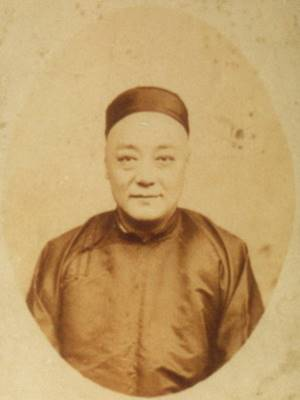
\includegraphics[width=3.5cm]{pengmingbao}
    \caption{彭名保}
   \end{figure}
  \end{column}
  \begin{column}{0.65\linewidth}
   \begin{itemize}
    \item 电话传入我国,是在1881年,英籍电气技师皮晓浦在上海十六铺沿街架起一对露天电话,付36文制钱可通话一次,这是中国的第一部电话。1882年2月,丹麦大北电报公司在上海外滩扬于天路办起我国第一个电话局,用户25家。
    \item 1889年,安徽省安庆州候补知州\textbf{彭名保},自行设计了一部电话,包括自制的五六十种大小零件,称为我国第一部自行设计制造的电话。
   \end{itemize}
  \end{column}
 \end{columns}
\end{frame}

\begin{frame}{电磁波的发现}
 % Electromagnetic wave - black
 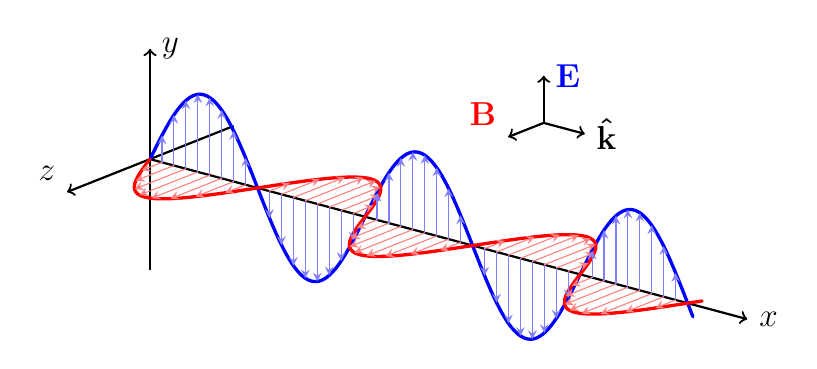
\begin{tikzpicture}[x=(-15:0.9), y=(90:1.0), z=(-150:1.0),
   line cap=round, line join=round,
   axis/.style={black, thick,->},
   vector/.style={>=stealth,->}]
  \large
  \def\A{1}
  \def\nNodes{5} % use even number
  \def\nVectorsPerNode{8}
  \def\N{\nNodes*40}
  \def\xmax{\nNodes*pi/2*1.01}
  \pgfmathsetmacro\nVectors{(\nVectorsPerNode+1)*\nNodes}

  \def\vE{{\color{blue}\mathbf{E}}}
  \def\vB{{\color{red}\mathbf{B}}}
  \def\vk{\mathbf{\hat{k}}}

  % main axes
  \draw[axis] (0,0,0) -- ++(\xmax*1.1,0,0) node[right] {$x$};
  \draw[axis] (0,-\A*1.4,0) -- (0,\A*1.4,0) node[right] {$y$};
  \draw[axis] (0,0,-\A*1.4) -- (0,0,\A*1.4) node[above left] {$z$};

  % small axes
  \def\xOffset{{(\nNodes-2)*pi/2}}
  \def\yOffset{\A*1.2}
  \def\zOffset{\A*1.2}
  \draw[axis] (\xOffset,\yOffset,-\zOffset) -- ++(\A*0.6,0,0) node[right] {$\vk$};
  \draw[axis] (\xOffset,\yOffset,-\zOffset) -- ++(0,\A*0.6,0) node[right] {$\vE$};
  \draw[axis] (\xOffset,\yOffset,-\zOffset) -- ++(0,0,\A*0.6) node[above left] {$\vB$};

  % equation
  %\node[above right] at (\xOffset,-0.5*\yOffset,4*\zOffset)
  %  {$\begin{aligned}
  %    \vE &= \mathbf{E_0}\sin(\vk\cdot\mathbf{x}-c_0t)\\
  %    \vB &= \mathbf{B_0}\sin(\vk\cdot\mathbf{x}-c_0t)\\
  %    \end{aligned}$};
  %\node[below right] at (\xOffset,-0.5*\yOffset,4*\zOffset)
  %  {$\vE\cdot\vk = 0,\;\; \vB\cdot\vk = 0,\;\; \vB = \frac{1}{c_0}\vk\times\vE$};

  % waves
  \draw[blue,very thick,variable=\t,domain=0:\nNodes*pi/2*1.01,samples=\N]
  plot (\t,{\A*sin(\t*360/pi)},0);
  \draw[red,very thick,variable=\t,domain=0:\nNodes*pi/2*1.01,samples=\N]
  plot (\t,0,{\A*sin(\t*360/pi)});

  % draw vectors
  \foreach \k [evaluate={\t=\k*pi/2/(\nVectorsPerNode+1);
     \angle=\k*90/(\nVectorsPerNode+1);
     \c=(mod(\angle,90)!=0);}]
  in {1,...,\nVectors}{
    \if\c1
     \draw[vector,blue!50] (\t,0,0) -- ++(0,{\A*sin(2*\angle)},0);
     \draw[vector,red!50] (\t,0,0) -- ++(0,0,{\A*sin(2*\angle)});
    \fi
   }
 \end{tikzpicture}
 \begin{itemize}
  \item 自从贝尔发明了电话机,这样人人都能手拿一个“话柄”,和远方的亲朋好友谈天说地了。电报和电话的相继发明,使人类获得了远距离传送信息的重要手段。但是,电信号都是通过金属线传送信息的重要手段。但是,电信号都是通过金属线传送的。线路架设到的地方,信息才能传到,这就大大限制了信息的传播范围,特别是在大海、高山,有没有能让信息\textbf{无线}传播的方法?
 \end{itemize}
\end{frame}

\begin{frame}{电磁波的发现}
 \begin{columns}
  \begin{column}{0.35\linewidth}
   \begin{figure}
    \includegraphics[width=3.5cm]{oersted.jpg}
    \caption{汉斯·克里斯蒂安·奥斯特 Hans Christian Oersted(1777 - 1851)}
   \end{figure}
  \end{column}
  \begin{column}{0.65\linewidth}
   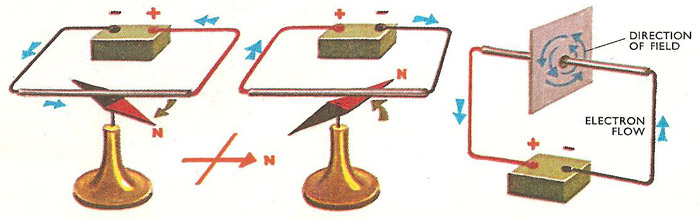
\includegraphics[width=6.5cm]{oerstedexperiment.jpg}
   \begin{itemize}
    \item 1820年,丹麦物理学家奥斯特发现电流磁效应
    \item 1934年以“奥斯特”命名CGS单位制中的磁场强度单位
   \end{itemize}
  \end{column}
 \end{columns}
\end{frame}

\begin{frame}{电磁波的发现}
 \begin{columns}
  \begin{column}{0.35\linewidth}
   \begin{figure}
    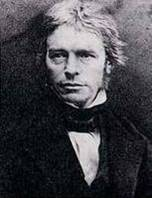
\includegraphics[width=3.5cm]{faraday.jpg}
    \caption{迈克尔·法拉第Michael Faraday(1791-1867)}
   \end{figure}
  \end{column}
  \hfill
  \begin{column}{0.65\linewidth}
   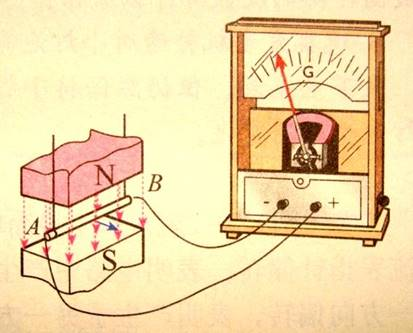
\includegraphics[width=5cm]{faradayexperiment.jpg}
   \begin{itemize}
    \item 英国物理学家、化学家
    \item 1831年发现电磁感应
   \end{itemize}
  \end{column}
 \end{columns}
\end{frame}

\begin{frame}{电磁波的发现}
 \begin{columns}
  \begin{column}{0.35\linewidth}
   \begin{figure}
    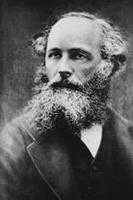
\includegraphics[width=3.5cm]{maxwell.jpg}
    \caption{詹姆斯·克拉克·麦克斯韦James Clerk Maxwell (1831-1879)}
   \end{figure}
  \end{column}
  \begin{column}{0.65\linewidth}
   Maxwell Equations:
   %\begin{equation}
   \begin{align*}
     & \nabla\times\vec E=-\frac{\partial \vec B}{\partial t}         \\
     & \nabla\times\vec H=\vec{J} +\frac{\partial \vec D}{\partial t} \\
     & \nabla\cdot\vec{D}=\rho                                        \\
     & \nabla\cdot\vec{B}=0
   \end{align*}
   %\end{equation}
   \begin{itemize}
    \item 英国物理学家。1864年,麦氏发表了电磁场理论,成为人类历史上预言电磁波存在的\textbf{第一人}
   \end{itemize}
  \end{column}
 \end{columns}
\end{frame}

\begin{frame}{电磁波的发现}
 \begin{columns}
  \begin{column}{0.35\linewidth}
   \begin{figure}
    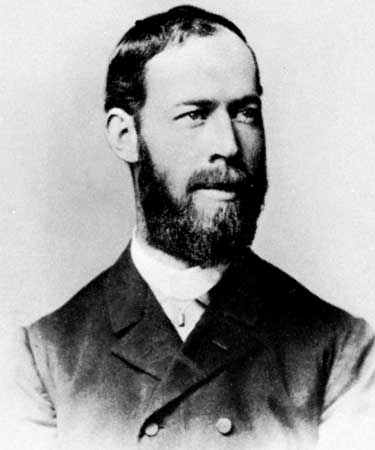
\includegraphics[width=3.5cm]{hertz.jpg}
    \caption{亨利希·鲁道夫·赫兹 Heinrich Hertz(1857 - 1894)}
   \end{figure}
  \end{column}
  \begin{column}{0.65\linewidth}
   \begin{figure}
    \flushright
    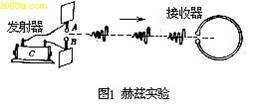
\includegraphics[width=3.5cm]{hertzexperiment.jpg}
   \end{figure}
   \begin{itemize}
    \item 德国物理学家,1887年,实验证实了电磁波的存在和传播。成为了近代科学技术史的一座里程碑,为了纪念这位杰出的科学家,电磁波的单位便命名为“赫兹($Hz$)”
    \item 证明了麦克斯韦理论的正确,导致了无线电的诞生,开辟了电子技术的新纪元,标志着从“有线电通信”向“无线电通信”的转折点。也是整个移动通信的发源点,应该说,从这时开始,人类开始进入了无线通信的新领域。
   \end{itemize}
  \end{column}
 \end{columns}
\end{frame}

\begin{frame}{无线电报的发明}
 \begin{columns}
  \begin{column}{0.35\linewidth}
   \begin{figure}
    \includegraphics[width=3.5cm]{popov.jpg}
    \caption{波波夫Popov, Aleksandr Stepanovic(1859 - 1906)}
   \end{figure}
  \end{column}
  \begin{column}{0.65\linewidth}
   \begin{figure}
    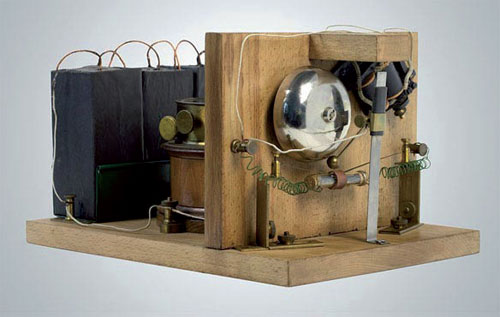
\includegraphics[width=6.5cm]{wirelessreceiver.jpg}
    \caption{1894年,发明了第一架无线电接收器}
   \end{figure}
  \end{column}
 \end{columns}
\end{frame}

\begin{frame}{无线电报的发明}
 \begin{columns}
  \begin{column}{0.35\linewidth}
   \begin{figure}
    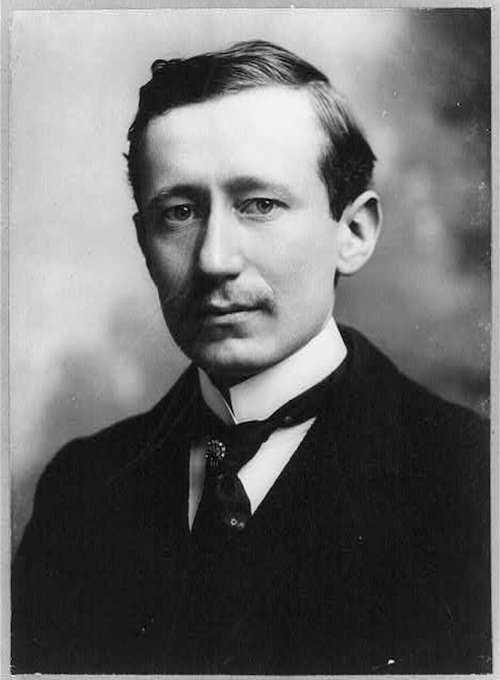
\includegraphics[width=3.5cm]{marconi2.jpg}
    \caption{伽利尔摩·马可尼 Guglielmo Marchese Marconi(1874 - 1937)}
   \end{figure}
  \end{column}
  \begin{column}{0.65\linewidth}
   \begin{itemize}
    \item 意大利无线电工程师,企业家,实用无线电报通信的创始人。
    \item 1897年,在伦敦成立“马可尼无线电报公司”。
    \item 1909年他与布劳恩一起获得诺贝尔物理学奖。
   \end{itemize}
  \end{column}
 \end{columns}
\end{frame}

\begin{frame}{无线电报的发明}
 由于无线电通信不需要昂贵的地面通信线路和海底电缆,因而很快便受到人们的重视。它首先被用于敷设线路困难的海上通信。第一艘装有无线电台的船只是美国的“圣保罗”号邮船。后来,海上无线电通信接二连三地在援救海上遇险船只的行动中发挥作用,从而崭露头角。让我们想起\textbf{波波夫}的那句话:\textbf{“要是我能指挥电磁波,就可飞越整个世界”。}
\end{frame}

\begin{frame}{无线电通信的发明}
 \begin{columns}
  \begin{column}{0.35\linewidth}
   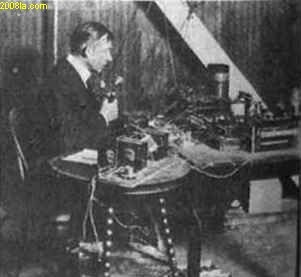
\includegraphics[width=3.5cm]{broadcast1.jpg}
  \end{column}
  \begin{column}{0.65\linewidth}
   \begin{itemize}
    \item 1906年12月24日平安夜,晚上8点左右,在美国新英格兰海岸附近穿梭往来的船只上,一些听惯了“滴滴嗒嗒”莫尔斯电码声的报务员们,忽然听到了耳机中传来有人正在朗诵圣经的故事,有人拉着小提琴,还伴奏有亨德尔的《舒缓曲》……。
   \end{itemize}
  \end{column}
 \end{columns}
\end{frame}

\begin{frame}{无线电通信的发明}
 \begin{columns}
  \begin{column}{0.35\linewidth}
   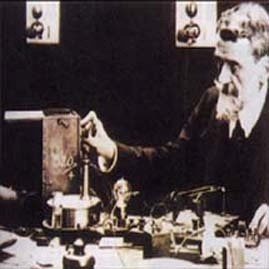
\includegraphics[width=3.5cm]{broadcast2.jpg}
  \end{column}
  \begin{column}{0.65\linewidth}
   \begin{itemize}
    \item 1902年美国人巴纳特·史特波菲德在肯塔基州穆雷市进行了第一次无线电广播。
    \item 1920年,美国匹兹堡的KDKA电台进行了首次商业无线电广播
   \end{itemize}
  \end{column}
 \end{columns}
\end{frame}

\begin{frame}{无线电通信的发明}
 \begin{columns}
  \begin{column}{0.35\linewidth}
   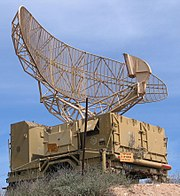
\includegraphics[width=3.5cm]{radar.jpg}
  \end{column}
  \begin{column}{0.65\linewidth}
   \begin{itemize}
    \item 与此同时,无线电通信逐渐被用于战争。在第一次和第二次世界大战中,它都发挥了很大的威力,以至于有人把第二次世界大战称为“无线电战争”。
   \end{itemize}
  \end{column}
 \end{columns}
\end{frame}

\subsection{微波及其特点}
\begin{frame}{微波及其特点}
 \begin{columns}
  \begin{column}{0.3\linewidth}
   %\begin{itemize}
   电磁波按波长(或频率)划分,则大致可以把$300MHz - 3000GHz$,(对应空气中波长$\lambda$是$1m - 0.1mm$)这一频段的电磁波称之为微波。它处于超短波和红外光波之间。
   %\end{itemize}
  \end{column}
  \begin{column}{0.7\linewidth}
   \tikzset{twoline/.style={align=center,execute at begin node=\setlength{\baselineskip}{0.5em}}}
   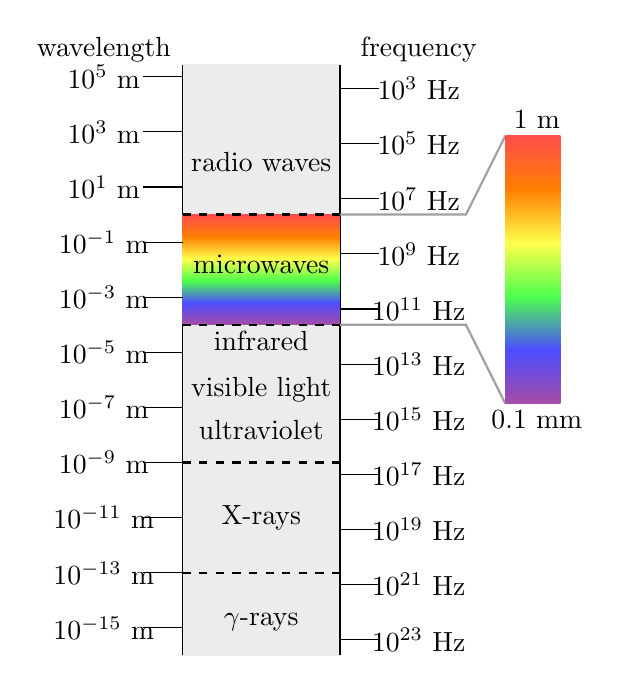
\begin{tikzpicture}
    % define visible spectrum shading
    \pgfdeclareverticalshading{visible}{100bp}
    {color(0bp)=(violet!70); color(25bp)=(violet!70); color(35bp)=(blue!70);
     color(45bp)=(green!70); color(55bp)=(yellow!70); color(65bp)=(orange);
     color(75bp)=(red!70); color(100bp)=(red!70)}
    % grayish background for spectrum labels
    \draw[gray!15,fill] (-1,0) rectangle (1,7.5);
    % axes
    \draw (-1,0) -- (-1,7.5) (1,0) -- (1,7.5);
    \node at (-2,7.7) {wavelength};
    \node at (2,7.7) {frequency};
    % spectrum labels
    \shade[shading=visible] (-1,4.2) rectangle (1,5.6);
    \foreach \x/\xlabel in {1.9/{radio waves}, -1.8/{microwaves}, -4.6/{infrared}, -6.35/{visible light}, -7.8/{ultraviolet}, -11/{X-rays}, -14.8/{$\gamma$-rays} } \node at (0,{\x*0.35+5.6}) {\xlabel};
    % values of wavelengths
    \foreach \x in {5,3,1,...,-15} {
      \draw (-1,{\x*0.35+5.6}) --++ (-0.5,0);
      \node at (-2,{\x*0.35+5.6}) {$10^{\x}$ m};
     }
    % values of frequencies
    \foreach \x in {3,5,...,23} {
      \draw (1,{-\x*0.35+8.25}) --++ (0.5,0);
      \node at (2,{-\x*0.35+8.25}) {$10^{\x}$ Hz};
     }
    % dashed lines as separators
    \foreach \x in {0,-4,-9,-13} \draw[dashed,thick] (-1,{\x*0.35+5.6}) --++ (2,0);
    % extension for visible spectrum
    \draw[thick, gray!75] (1,4.2) --++ (1.6,0) -- (3.1,3.2);
    \draw[thick, gray!75] (1,5.6) --++ (1.6,0) -- (3.1,6.6);
    \shade[shading=visible] (3.1,3.2) rectangle (3.8,6.6);
    \node at (3.5, 6.8) {1 m};
    \node at (3.5, 3.0) {0.1 mm};
    %\node[right] at (3.5, 6.4) {1 m};
    %\node[right] at (3.5, 3.4) {0.1 mm};
   \end{tikzpicture}
  \end{column}
 \end{columns}
\end{frame}

\begin{frame}{微波波段的划分}
 \begin{tabular}{cccc}
  \toprule
  波段代号 & 标称波长/cm & 频率范围/GHz & 波长范围/cm \\
  \midrule
  L        & 22          & 1-2          & 30-15       \\
  S        & 10          & 2-4          & 15-7.5      \\
  C        & 5           & 4-8          & 7.5-3.5     \\
  X        & 3           & 8-12         & 3.75-2.5    \\
  Ku       & 2           & 12-18        & 2.5-1.67    \\
  K        & 1.25        & 18-27        & 1.67-1.11   \\
  Ka       & 0.8         & 27-40        & 1.11-0.75   \\
  U        & 0.6         & 40-60        & 0.75-0.5    \\
  V        & 0.4         & 60-80        & 0.5-0.375   \\
  W        & 0.3         & 80-100       & 0.375-0.3   \\
  \bottomrule
 \end{tabular}
\end{frame}

\begin{frame}{Maxwell方程组的物理意义}
 \begin{columns}
  \begin{column}{0.4\linewidth}
   \begin{align*}
     & \nabla\times\vec{E} = -\frac{\partial \vec{B}}{\partial t}        \\
     & \nabla\times\vec{H} = \vec{J}+\frac{\partial \vec{D}}{\partial t}
   \end{align*}
  \end{column}
  \begin{column}{0.6\linewidth}
   \begin{itemize}
    \item 这两个方程左边物理量为磁(或电),而右边物理量则为电(或磁)。这中间的等号深刻揭示了电与磁的相互转化,相互依赖,相互对立,共存于统一的电磁波中。正是由于电不断转换为磁,而磁又不断转换成为电,才会发生能量交换和贮存。
   \end{itemize}
  \end{column}
 \end{columns}
 \centering
 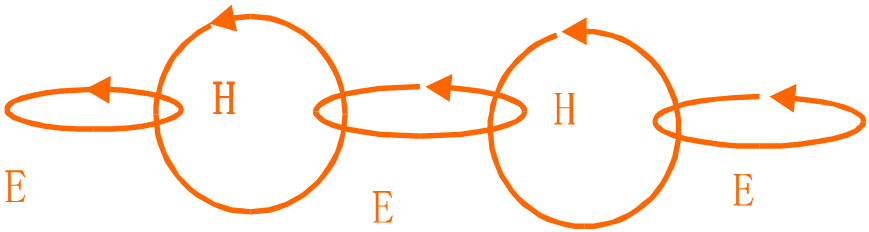
\includegraphics[width=6.5cm]{ehconvert.png}
\end{frame}

\begin{frame}{电与磁的转换}
 \begin{itemize}
  \item Oersted和Faraday的实验证实了电磁转换,而且还知道了只有动磁才能转化为电。
  \item 还需提到:电磁转换为电磁波的出现提供了可能,但不一定是现实。例如电磁振荡也是典型的电磁转换,但没有引起\textbf{波(Wave)}。
  \item 作为力学类比,电磁转换犹如单摆问题中的动能与势能的转化。
 \end{itemize}
 \begin{columns}
  \begin{column}{0.45\linewidth}
   \begin{figure}
    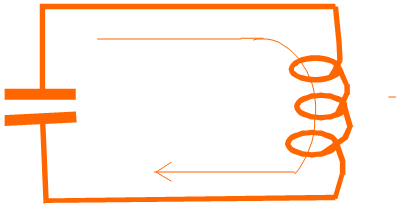
\includegraphics[width=4cm]{oscillator.png}
    \caption{电磁振荡}
   \end{figure}
  \end{column}
  \begin{column}{0.45\linewidth}
   \begin{figure}
    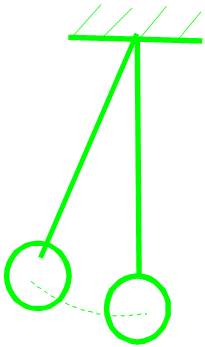
\includegraphics[width=1.8cm]{pendulum.png}
    \caption{单摆}
   \end{figure}
  \end{column}
 \end{columns}
\end{frame}

\begin{frame}{Maxwell方程组的物理意义}
 \begin{itemize}
  \item 进一步研究Maxwell方程两边的运算,从物理上看,运算反映一种作用(Action)。方程左边是空间运算(\textbf{旋度});方程右边是时间运算(\textbf{导数}),中间用等号连接。它深刻揭示了电(或磁)场任一地点的变化会转化为磁(或电)场时间的变化;反过来,场的时间变化也会转化成地点的变化。正是这种空间和时间的相互变化构成了波动的外在形式。用通俗的一句话说:即\textbf{一个地点出现过的事物,过了一段时间又在另一地点出现了}。
 \end{itemize}
\end{frame}

\begin{frame}{Maxwell方程组的物理意义}
 \begin{itemize}
  \item Maxwell方程还指出:电磁转化有一个重要条件,即频率$\omega$。只有较高的$\omega$才能确保电磁的有效转换,直流情况没有转换。可以这样说,在高频封闭电路才有可能变成开放电路。不过很有意思的是频率越高,越难输出功率,这也是一个有趣的矛盾。
        \begin{columns}
         \begin{column}{0.4\linewidth}
          \begin{align*}
            & \nabla\times\vec{H} = \mathrm{j}\omega\epsilon\vec{E}+\vec{J} \\
            & \nabla\times\vec{E} = -\mathrm{j}\omega\mu\vec{H}
          \end{align*}
         \end{column}
         \begin{column}{0.6\linewidth}
          \textbf{单色波}频域的Maxwell方程
         \end{column}
        \end{columns}
 \end{itemize}
\end{frame}

\begin{frame}{Maxwell方程组的物理意义}
 \begin{columns}
  \begin{column}{0.4\linewidth}
   \begin{align*}
     & \nabla\times\vec E=-\frac{\partial \vec B}{\partial t}         \\
     & \nabla\times\vec H=\vec{J} +\frac{\partial \vec D}{\partial t} \\
     & \nabla\cdot\vec{D}=\rho                                        \\
     & \nabla\cdot\vec{B}=0
   \end{align*}
  \end{column}
  \begin{column}{0.65\linewidth}
   \begin{itemize}
    \item 在Maxwell方程中还存在另一对矛盾对抗,这就构成了Maxwell方程本质的不对称性。尽管为了找其对称性而一直在探索磁流$\vec{M}$的存在,但到目前为止始终未果。
   \end{itemize}
  \end{column}
 \end{columns}
\end{frame}

\begin{frame}{微波的特点}
 \begin{enumerate}
  \item 微波的两重性\\ 微波的两重性指的是对于尺寸大的物体,如大型建筑物、山谷等它显示出粒子的特点——即似光性或直线性,而对于相对尺寸小的物体,又显示出——波动性或似声性。
  \item 微波与“左邻右舍”的比较\\ 微波的“左邻”是超短波和短波,而它的“右舍”又是红外光波。
        \saveenum
 \end{enumerate}
 \begin{columns}
  \begin{column}{0.44\linewidth}
   \begin{tcolorbox}[colback=blue!5,colframe=blue!40!black,title=微波与超短波、短波比较]
    微波与超短波、短波相比较大大扩展了通讯通道,开辟了微波通讯和卫星通讯。
   \end{tcolorbox}
  \end{column}
  \begin{column}{0.55\linewidth}
   \begin{tcolorbox}[colback=blue!5,colframe=blue!40!black,title=微波与光波比较]
    微波与光波比较,光通过雨雾衰减很大,特别是雾天,蓝光、紫光几乎看不见,这正是采用红光作警戒的原因。而微波波段穿透力强。
   \end{tcolorbox}
  \end{column}
 \end{columns}
\end{frame}

\begin{frame}{微波的特点}
 \begin{enumerate}
  \resume
  \item 宇宙“窗口”\\地球的外层空间由于日光等繁复的原因形成独特的电离层,它对于短波几乎全反射,这就是短波的天波通讯方式。因而在微波波段则有若干个可以通过电离层的“宇宙窗口”。因而微波是独特的宇宙通讯手段。
        \saveenum
 \end{enumerate}
 \centering
 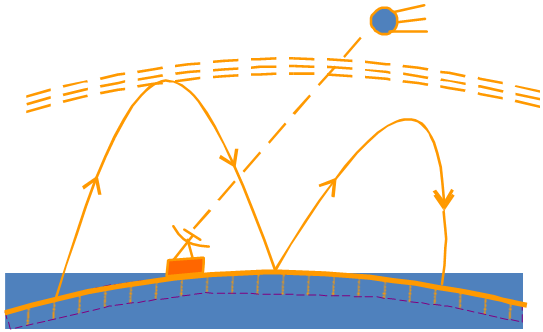
\includegraphics[width=6.5cm]{cosmicwindow.png}
\end{frame}

\begin{frame}{微波的特点}
 \begin{enumerate}
  \resume
  \item 计算机的运算次数进入十亿次,其频率也是微波频率。超高速集成电路的互耦也是微波互耦问题,因此,微波的研究已进入集成电路和计算机。
  \item 微波研究方法主要有两种:场论的研究方法和网络的研究方法。这也是本门课程要学习的重要方法。其中场论方法的基础是本征模理论。网络方法的基础是广义传输线理论。
 \end{enumerate}
\end{frame}

\subsection{微波的应用}
\begin{frame}{微波技术的应用及发展}
 \begin{itemize}
  \item 微波技术的应用\\
        \tikz [nodes={text height=.7em,text depth=.2em,draw=black!20,thick,fill=white},>={Stealth[round,sep]},rounded corners,semithick]
        \graph [layered layout,level distance=1cm,sibling sep=.5em,sibling distance=1cm]{
        微波应用 -> {雷达,通信,科学研究,生物医药,微波能};
        };
  \item 微波技术的发展\\
        \tikz [nodes={text height=.7em,text depth=.2em,draw=black!20,thick,fill=white},>={Stealth[round,sep]},rounded corners,semithick]
        \graph [layered layout,level distance=1cm,sibling sep=.5em,sibling distance=1cm]{
        发展方向 -> {工作频段向高频段发展,小型化宽带化,自动化智能化};
        };
 \end{itemize}
\end{frame}

\subsection{本课程内容}
\begin{frame}{本课程内容}
 \begin{columns}
  \begin{column}{0.2\linewidth}
   \begin{enumerate}
    \item 绪论
    \item 低频电路 $\longrightarrow$ 微波分析
          \saveenum
   \end{enumerate}
  \end{column}
  \begin{column}{0.3\linewidth}
   \textcolor{blue}{均匀传输线和波导理论基础}\\
   \textcolor{blue}{微波电路元件}
  \end{column}
  \begin{column}{0.5\linewidth}
   \begin{enumerate}
    \resume
    \item \textbf{分布电路与传输线理论}
    \item \textbf{Smith圆图和阻抗匹配}
    \item \textbf{微波网络理论}
    \item \textbf{实用微波传输线与波导}
    \item 微波谐振器
    \item \textbf{功率分配器和定向耦合器}
    \item 微波滤波器
   \end{enumerate}
  \end{column}
 \end{columns}
\end{frame}

\begin{frame}{微波技术的研究方法}
 \begin{tikzpicture}[
   terminal/.style={
     % The shape:
     rectangle,
     % The size:
     minimum size = 4mm,
     % The border:
     very thick,
     %draw=red!50!black!50, % 50% red and 50% black,
     % and that mixed with 50% white
     draw=blue!50,
     % The filling:
     %top color=white,      % a shading that is white at the top...
     %bottom color=red!50!black!20, % and something else at the bottom
     fill=white,
     % Fonts
     font=\itshape}]

  \node (W) [terminal]                                         {研究方法基本内容};
  \node (N) [terminal,above right=of W,xshift=0mm,yshift=4mm]  {麦克斯韦方程};
  \node (S) [terminal,below right=of W,xshift=0mm,yshift=-4mm] {基尔霍夫定律};
  \node (E) [terminal,below right=of N,xshift=0mm,yshift=-4mm] {场与路相结合};
  \draw [->] (W.north) .. controls +(up:10mm) and +(left:10mm) .. node[swap]{场} (N.west);
  \draw [->] (W.south) .. controls +(down:10mm) and +(left:10mm) .. node[swap]{路}(S.west);
  \draw [->] (N.east) .. controls +(right:10mm) and +(up:10mm) .. (E.north);
  \draw [->] (S.east) .. controls +(right:10mm) and +(down:10mm) .. (E.south);
 \end{tikzpicture}
\end{frame}

\subsection{导行波及其传输特性}
\begin{frame}{基本概念}
 \begin{enumerate}
  \item \textbf{导行系统(Guided system)}
        \saveenum
        \\约束或导引电磁能量定向传播\\
        作用:\\
        \begin{itemize}
         \item 无辐射损耗的将电磁波从一处传到另一处
         \item 设计成微波元件:滤波器、阻抗变换器、定向耦合器等。
        \end{itemize}
        微波电路是一种由各种导行系统构成的导行电磁波电路
 \end{enumerate}

\end{frame}

\begin{frame}{导行系统结构}
 %\begin{figure}
 \centering
 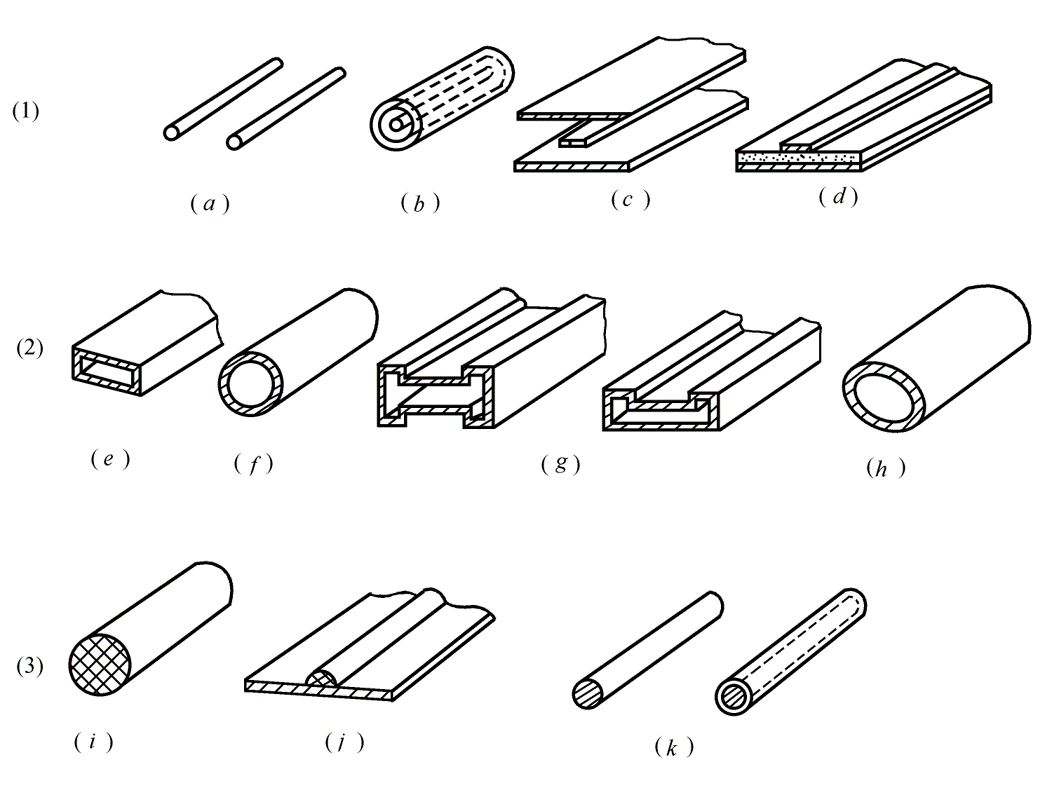
\includegraphics[width=9cm]{guidesystem.png}
 %\end{figure}
\end{frame}

\begin{frame}{基本概念}
 \begin{enumerate}
  \resume
  \item \textbf{导行波(Guided Wave)}
        \\沿导行系统定向传播的电磁波(导波)
        \\\textbf{TEM波}\quad 横电磁波 —— 各种传输线 电磁能量约束或限制在导体之间的空间内沿其轴向传播
        \\\textbf{TE/TM波}\quad 横电/横磁波 —— 封闭金属波导 电磁能量完全限制在金属管内沿轴向传播
        \\\textbf{表面波} —— 开波导 电磁能量约束在波导结构的周围(波导内和波导表面附近)沿轴向传播
        \saveenum
 \end{enumerate}
\end{frame}

\begin{frame}{基本概念}
 \begin{enumerate}
  \resume
  \item \textbf{导模(Guided mode)}
        \\导行波的模式(传输模)
        \\ *在导行系统横截面上的电磁场呈驻波分布,且完全确定的,与位置和频率无关
        \\ *导模是离散的,当频率一定时,每个导模具有唯一的传播常数
        \\ *导模之间相互正交,彼此独立,互不耦合
        \\ *具有截止特性,截止条件和截止波长因导行系统和模式而异
  \item \textbf{规则导行系统(Regular guided system)}
        \\无限长笔直导行系统,其横截面尺寸、媒质分布、结构材料、边界条件沿轴向均不变化
 \end{enumerate}
\end{frame}

\begin{frame}{导波场的分析}
 在\textbf{均匀}、\textbf{无耗}、\textbf{各向同性}、\textbf{无源}导行系统中
 \begin{columns}
  \begin{column}{0.5\linewidth}
   \begin{empheq}[box=\widefbox]{align*}
    &\nabla\times\vec E=-\frac{\partial \vec B}{\partial t}\\
    &\nabla\times\vec H=\frac{\partial \vec D}{\partial t}\\
    &\nabla\cdot\vec{D}=0\\
    &\nabla\cdot\vec{B}=0
   \end{empheq}
   设导波沿$z$向传播,坐标$z$与横向坐标无关
  \end{column}
  \begin{column}{0.5\linewidth}
   \flushright
   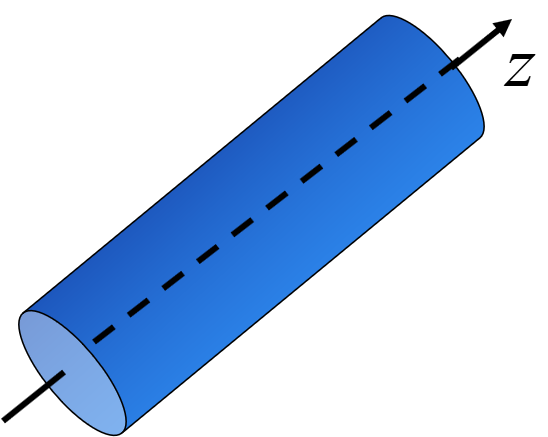
\includegraphics[width=4cm]{zuobiao.png}
   \begin{align*}
     & \nabla=\nabla_{t}+\hat z \partial / \partial z \\
     & \vec E=\vec E_{t}+\hat z E_{z}                 \\
     & \vec H=\vec H_{t}+\hat z H_{z}
   \end{align*}
  \end{column}
 \end{columns}
\end{frame}

\newcommand{\mtikzmark}[1]{\tikz[overlay,remember picture]\node(#1){};}
\tikzset{mylabel/.style={align=center,fill=blue!10,font=\footnotesize}}
%\mytlabel[options]{start.mark}{end.mark}{text}
\newcommand\mytlabel[4][]{%
 \tikz[overlay,remember picture]
 {\draw[->]([yshift=-10pt]#2.north) -- node[mylabel,#1]{#4}([yshift=6pt]#3.north);}
}
\begin{frame}{导波场的分析}
 \begin{columns}
  \begin{column}{0.45\linewidth}
   \begin{empheq}[box=\widefbox]{align*}
    %\tikzmarkin{c}(0.05,-0.6)(-0.05,0.65)
    & \nabla_t\times\vec{H_{t}}=\mathrm{j}\omega\epsilon\hat{z}E_{z} \\
    & \nabla_t\times\hat{z}H_{z}+\hat{z}\times\frac{\partial\vec{H_{t}}}{\partial z}
    = \mtikzmark{a}\mathrm{j}\omega\epsilon\vec{E_{t}}
   \end{empheq}
   %$$\times j\omega\mu$$
  \end{column}
  \begin{column}{0.5\linewidth}
   \begin{empheq}[box=\widefbox]{align*}
    & \nabla_t\times\vec E_{t}=-\mathrm{j}\omega\mu\hat{z} H_{z} \\
    & \nabla_t\times \hat z E_{z}+\hat{z}\times\mtikzmark{c}\frac{\partial\vec{E_{t}}}{\partial z}
    = -\mathrm{j}\omega\mu\vec{H_t}
   \end{empheq}
  \end{column}
 \end{columns}
 \begin{flalign*}
   & \mathrm{j}\omega\mu\hat{z}\times\frac{\partial \vec{H_{t}}}{\partial z}=\mtikzmark{b}-\mathrm{j}\omega\mu\nabla_{t}\times\hat{z}H_{z}-\omega^{2}\mu\epsilon\vec{E_{t}} &
 \end{flalign*}
 \begin{flalign*}
   &  & -\mathrm{j}\omega\mu\hat{z}\times\frac{\partial \vec{H_{t}}}{\partial z}=\hat{z}\times\frac{\partial}{\partial z} \left(\nabla_{t}\times\hat{z}E_{z}\right)+\hat{z}\times\mtikzmark{d}\frac{\partial}{\partial z} \left(\hat{z} \times \frac{\partial \vec{E_{t}}}{\partial z} \right)
 \end{flalign*}
 % draw arrow with text from specified position to another
 \mytlabel{a}{b}{$\times \mathrm{j}\omega\mu$}
 \mytlabel{c}{d}{$\hat{z}\times\frac{\partial}{\partial z}$}
\end{frame}

\begin{frame}{导波场的分析}
 \begin{empheq}[box=\widefbox]{align*}
  \left( k^{2}+\frac{\partial^{2}}{\partial z^{2}} \right)\vec{E_{t}}=\frac{\partial}{\partial z}\nabla_{t}E_{z}-\mathrm{j}\omega\mu\nabla_{t}\times\hat{z}H_{z}
 \end{empheq}
 \begin{empheq}[box=\widefbox]{align*}
  \left( k^{2}+\frac{\partial^{2}}{\partial z^{2}} \right)\vec{H_{t}}=\frac{\partial}{\partial z}\nabla_{t}H_{z}+\mathrm{j}\omega\epsilon\nabla_{t}\times\hat{z}E_{z}
 \end{empheq}
 在规则导行系统中,导波场的\textbf{横向分量}可用\textbf{纵向分量}完全确定。\\上面公式中$k^{2}=\omega^{2}\mu\epsilon$
\end{frame}

\begin{frame}{导波场的分析}
 \begin{empheq}[box=\widefbox]{align*}
  & \nabla^{2}\vec{E}+k^{2}\vec{E}=0\\
  & \nabla^{2}\vec{H}+\mtikzmark{a}k^{2}\vec{H}=0
 \end{empheq}
 \begin{columns}
  \begin{column}{0.45\linewidth}
   \begin{empheq}[box=\widefbox]{align*}
    & \nabla^{2}E_{z}+\mtikzmark{b}k^{2}E_{z}=0\\
    & \nabla^{2}H_{z}+\mtikzmark{d}k^{2}H_{z}=0
   \end{empheq}
  \end{column}
  \begin{column}{0.45\linewidth}
   \begin{empheq}[box=\widefbox]{align*}
    & \nabla^{2}\vec{E}_{t}+\mtikzmark{c}k^{2}\vec{E}_{t}=0\\
    & \nabla^{2}\vec{H}_{t}+k^{2}\vec{H}_{t}=0
   \end{empheq}
  \end{column}
 \end{columns}
 \flushright
 \begin{empheq}[box=\widefbox]{align*}
  \left( \nabla^{2}_{t}+\frac{\partial^{2}}{\partial z^{2}}\right)
  \left\{\begin{aligned}
   \mtikzmark{e}E_{z}(z,t) \\H_{z}(z,t)
  \end{aligned}\right\}
  +k^{2}
  \left\{\begin{aligned}
   E_{z}(z,t) \\H_{z}(z,t)
  \end{aligned}\right\}
  =0
 \end{empheq}
 \mytlabel{a}{b}{纵向场}
 \mytlabel{a}{c}{横向场}
 \mytlabel{d}{e}{Helmholtz Equation}
\end{frame}

\begin{frame}{导波场的分析}
 \begin{empheq}[box=\widefbox]{align*}
  \left( \nabla^{2}_{t}+\frac{\partial^{2}}{\partial z^{2}}\right)
  \left\{\begin{aligned}
   \mtikzmark{e}E_{z}(z,t) \\H_{z}(z,t)
  \end{aligned}\right\}
  +k^{2}
  \left\{\begin{aligned}
   E_{z}(z,t) \\H_{z}(z,t)
  \end{aligned}\right\}
  =0
 \end{empheq}
 \begin{enumerate}
  \item \textbf{分离变量法}\\
        令$E_{z}(z,t)=Z(z)E_{0z}(t)$ \\
        \begin{align*}
         \frac{\nabla_{t}^{2}E_{0z}(t)}{E_{0z}(t)}+\frac{d^{2}Z(z)/dz^{2}}{Z(z)}=-k^{2}
        \end{align*}
        \begin{columns}
         \begin{column}{0.3\linewidth}
          分离变量常数: $k_{c}$和$\beta$
         \end{column}
         \begin{column}{0.6\linewidth}
          \begin{empheq}[box=\widefbox]{align*}
           & d^{2}Z(z)/dz^{2}+\beta^{2}Z(z)=0 \\
           & \nabla_{t}^{2}E_{0z}(t)+k_{c}^{2}E_{0z}(t)=0
          \end{empheq}
          \flushright————本征值方程
         \end{column}
        \end{columns}
        \saveenum
 \end{enumerate}
\end{frame}

\begin{frame}{导波场的分析}
 \begin{enumerate}
  \resume
  \item \textbf{色散关系}
        \begin{columns}
         \begin{column}{0.55\linewidth}
          \begin{empheq}[box=\widefbox]{align*}
           & k^{2}=k_{c}^{2}+\beta^{2}\\
           & \beta=\sqrt{k^{2}-k_{c}^{2}}=k\sqrt{1-(k_{c}/k)^{2}}
          \end{empheq}
         \end{column}
         \begin{column}{0.4\linewidth}
          \raggedright
          $k^{2}=\omega^{2}\mu\epsilon$\\  $\beta$:导波的传播常数或相移常数
         \end{column}
        \end{columns}
        $$d^{2}Z(z)/dz^{2}+\beta^{2}Z(z)=0$$
        %\flushleft
        解:
        \begin{empheq}[box=\widefbox]{align*}
         Z(z)=A_{1}exp(-\mathrm{j}\beta z)+A_{2}exp(\mathrm{j}\beta z)
        \end{empheq}
        \textbf{规则导行系统中沿正$z$方向传播的导波纵向场分量}\\
        \begin{align*}
         E_{z}(t,z)=E_{0z}(t)exp(-\mathrm{j}\beta z) \\
         H_{z}(t,z)=H_{0z}(t)exp(-\mathrm{j}\beta z)
        \end{align*}
        \saveenum
 \end{enumerate}
\end{frame}

\begin{frame}{导波场的分析}
 \begin{enumerate}
  \resume
  \item 本征值方程
        \begin{empheq}[box=\widefbox]{align*}
         \nabla_{t}^{2}E_{0z}(t)+k_{c}^{2}E_{0z}(t)=0
        \end{empheq}
        $k_{c}$:在特定边界条件下的本征值,称为导波的横向截止波数\\
        $k_{c}\neq 0$
        \saveenum
 \end{enumerate}
\end{frame}

\begin{frame}{导波场的分析}
 \begin{enumerate}
  \resume
  \item 横-纵向场的关系
        \begin{empheq}[box=\widefbox]{align*}
         \left( k^{2}+\frac{\partial^{2}}{\partial z^{2}}\right)\vec{E}_{t}=\frac{\partial}{\partial z}\nabla_{t}E_{z}-\mathrm{j}\omega\mu\nabla_{t}\times\hat{z}H_{z}\\
         \left( k^{2}+\frac{\partial^{2}}{\partial z^{2}}\right)\vec{H}_{t}=\frac{\partial}{\partial z}\nabla_{t}H_{z}+\mathrm{j}\omega\epsilon\nabla_{t}\times\hat{z}E_{z}
        \end{empheq}
        \begin{columns}
         \begin{column}{0.6\linewidth}
          \begin{empheq}[box=\widefbox]{align*}
           \vec{E}_{t}=\frac{-\mathrm{j}\beta}{k_{c}^{2}}\left[\nabla_{t}E_{z}+Z_{h}\nabla_{t}H_{z}\times\hat{z}\right]\\
           \vec{H}_{t}=\frac{-\mathrm{j}\beta}{k_{c}^{2}}\left[\nabla_{t}H_{z}+Y_{e}\hat{z}\times\nabla_{t}E_{z}\right]
          \end{empheq}
         \end{column}
         \begin{column}{0.4\linewidth}
          \begin{align*}
           Z_{h}=\sqrt{\frac{\mu}{\epsilon}}\frac{k}{\beta} \\
           Y_{e}=\sqrt{\frac{\epsilon}{\mu}}\frac{k}{\beta}
          \end{align*}
         \end{column}
        \end{columns}
        \saveenum
 \end{enumerate}
\end{frame}

\begin{frame}{导波场的分析}
 \begin{enumerate}
  \resume
  \item 导波的种类\\
        \begin{block}{横磁波(TM)或电(E)波——$H_{z}=0$}
         \begin{empheq}[box=\widefbox]{align*}
          \vec{E}_{t}^{e}=\frac{-\mathrm{j}\beta}{k_{c}^{2}}\nabla_{t}E_{z}\qquad
          \vec{H}_{t}^{e}=\frac{-\mathrm{j}\beta}{k_{c}^{2}}Y_{e}\hat{z}\times\nabla_{t}E_{z}
         \end{empheq}
        \end{block}
        \begin{block}{横电波(TE)或磁(H)波——$E_{z}=0$}
         \begin{empheq}[box=\widefbox]{align*}
          \vec{E}_{t}^{h}=\frac{-\mathrm{j}\beta}{k_{c}^{2}}Z_{h}\nabla_{t}H_{z}\times\hat{z}\qquad
          \vec{H}_{t}^{h}=\frac{-\mathrm{j}\beta}{k_{c}^{2}}\nabla_{t}H_{z}
         \end{empheq}
        \end{block}
        导行系统横向为调谐(振动)解形式$k_{c}^{2}>0$,$k^{2}>\beta^{2}$;$\beta=k\cdot\sqrt{1-\left(k_{c}/k\right)^{2}}$ 相速$v_{p}>c/\sqrt{\epsilon_{r}}$快波,有色散性,且需满足$k_{c}<k$才能传播。
 \end{enumerate}
\end{frame}

\begin{frame}{导波场的分析}
 \begin{block}{横电磁波(TEM)——$E_{z}=H_{z}=0$}
  %\begin{flalign*}
  $$ \because E_{t}\neq 0,H_{t}\neq 0 $$
  %\end{flalign*}
  以及
  \begin{align*}
    & \vec{E}_{t}=\frac{-\mathrm{j}\beta}{k_{c}^{2}}[\nabla_{t}E_{z}+Z_{h}\nabla_{t}H_{z}\times\hat{z}] \\
    & \vec{H}_{t}=\frac{-\mathrm{j}\beta}{k_{c}^{2}}[\nabla_{t}H_{z}+Y_{e}\hat{z}\times\nabla_{t}E_{z}]
  \end{align*}
  $$\left(\frac{0}{0}\right)\text{形式}\Longrightarrow k_{c}=0 \qquad k^{2}=k_{c}^{2}+\beta^{2}\Longrightarrow \beta=k $$
 \end{block}
\end{frame}

\begin{frame}{导波场的分析}
 又由$\nabla_{t}\times\vec{E}_{t}=-\mathrm{j}\omega\mu\hat{z}H_{z}$\qquad$\nabla_{t}\times\vec{H}_{t}=\mathrm{j}\omega\epsilon\hat{z}E_{z}$
 \begin{empheq}[box=\widefbox]{align*}
  \nabla_{t}\times\vec{E}_{t}^{0}=0 \qquad \nabla_{t}\times\vec{H}_{t}^{0}=0
 \end{empheq}
 $$\nabla_{t}\times\hat{z}E_{z}+\hat{z}\times\frac{\partial\vec{E}_{t}}{\partial z}=-\mathrm{j}\omega\mu\vec{H}_{t} \qquad \nabla_{t}\times\hat{z}H_{z}+\hat{z}\times\frac{\partial\vec{H}_{t}}{\partial z}=\mathrm{j}\omega\epsilon\vec{E}_{t} $$
 \begin{columns}
  \begin{column}{0.2\linewidth}
   \begin{empheq}[box=\widefbox]{align*}
    & \frac{\partial}{\partial z}=-\mathrm{j}\beta \\ & k=\omega\sqrt{(\mu\epsilon)}
   \end{empheq}
  \end{column}
  \begin{column}{0.75\linewidth}
   \begin{empheq}[box=\widefbox]{align*}
    \vec{E}_{t}^{0}\times \hat{z}=-\eta\vec{H}_{t}^{0} \qquad \eta\vec{H}_{t}^{0}\times\hat{z}=\vec{E}_{t}^{0}\quad \text{TEM波}
   \end{empheq}
  \end{column}
 \end{columns}
 \begin{columns}
  \begin{column}{0.4\linewidth}
   固有阻抗$\eta=\sqrt{(\mu/\epsilon)}\text{且}$
  \end{column}
  \begin{column}{0.5\linewidth}
   \begin{empheq}[box=\widefbox]{align*}
    \nabla_{t}^{2}\vec{E}_{0t}^{0}(t)=0 \quad \nabla_{t}^{2}\vec{H}_{0t}^{0}(t)=0
   \end{empheq}
  \end{column}
 \end{columns}
 TEM的导波场与静态场相同,存在于导体之间,或由双导体或多导体构成的导行系统(传输线)中,故又称为传输线模式;导波的相速、群速与无耗媒质平面波相同,无色散现象。
\end{frame}

\begin{frame}{导波场的分析}
 混合波\quad——\quad\fbox{$k_{c}^{2}<0$}\\导行系统横向为衰减解形式,场被束缚在导行系统表面——表面波可存在于电抗壁导行系统中,例如:介质波导、光纤等。
 \begin{empheq}[box=\widefbox]{align*}
  k^{2}<\beta^{2}\rightarrow v_{p}<c/\sqrt{\epsilon_{r}}
 \end{empheq}
 \textbf{称为慢波,且需满足$k_{c}<k$才能传播}
\end{frame}

\begin{frame}{导行波的一般传输特性}
 \begin{enumerate}
  \item \textbf{导模的截止波长与传输条件}\\
        导行系统中某导模无衰减能传播的最大波长——\textbf{截止波长}$\lambda_{c}$ \\
        导行系统中某导模无衰减能传播的最小频率——\textbf{截止频率}$f_{c}$ \\
        导波的传播常数\quad \widefbox{$\beta=k\sqrt{1-(k_{c}/k)^{2}}$} \\
        为虚数时,导模不能传播。\\
        当$k^{2}=\omega^{2}\mu\epsilon=k_{c}^{2}$时$\beta=0$,导模截止。\\
        对应的截止频率\quad$\Longrightarrow$\quad $\omega\sqrt{\mu\epsilon}=k_{c}$ \\
        \begin{empheq}[box=\widefbox]{align*}
         & \textbf{截止频率:}f_{c}=\frac{k_{c}}{2\pi\sqrt{\mu\epsilon}}\\
         & \textbf{截止波长:}\lambda_{c}=\frac{2\pi}{k_{c}}
        \end{empheq}
        \saveenum
 \end{enumerate}
\end{frame}

\begin{frame}{导行波的一般传输特性}
 \begin{enumerate}
  \resume
  \item \textbf{相速度和群速度}\\
        相速度:导模等相位面移动速度
        \begin{empheq}[box=\widefbox]{align*}
         & v_{p}=\frac{\omega}{\beta}=\frac{\omega}{k}
         \frac{1}{\sqrt{1-(k_{c}/k)^{2}}}
         =\frac{v}{\sqrt{1-(\lambda/\lambda_{c})^{2}}}=\frac{v}{G}\\
         & \text{平面波在介质中光速:}v=c/\sqrt{\epsilon_{r}}\\
         & \text{色散因子:}G=\sqrt{1-(\lambda/\lambda_{c})^{2}}
        \end{empheq}
        群速度:波包移动速度或窄带信号移送速度
        \begin{empheq}[box=\widefbox]{align*}
         v_{g}=\frac{d\omega}{d\beta}=v\sqrt{1-(\lambda/\lambda_{c})^{2}}=vG
        \end{empheq}
        \begin{empheq}[box=\widefbox]{align*}
         v_{p}\cdot v_{g}=v^{2}
        \end{empheq}
        \saveenum
 \end{enumerate}
\end{frame}

\begin{frame}{导行波的一般传输特性}
 \begin{enumerate}
  \resume
  \item \textbf{波导波长}\\
        导行系统中导模相邻同相位面之间距离,或者相位差2$\pi$的相位面之间的距离。\\
        \begin{empheq}[box=\widefbox]{align*}
         \lambda_{g}=\frac{2\pi}{\beta}=\frac{\lambda}{\sqrt{1-(\lambda/\lambda_{c})^{2}}}
        \end{empheq}
  \item \textbf{波阻抗}\\
        导模的横向电场和横向磁场之比\\
        \begin{empheq}[box=\widefbox]{align*}
         & Z_{TE}=\frac{E_{u}}{H_{v}}=\frac{-E_{v}}{H_{u}}=\frac{\omega\mu}{\beta}=\frac{\eta}{\sqrt{1-(\lambda/\lambda_{c})^{2}}}\\
         & Z_{TM}=\frac{E_{u}}{H_{v}}=\frac{-E_{v}}{H_{u}}=\frac{\beta}{\omega\mu}=\eta\sqrt{1-(\lambda/\lambda_{c})^{2}}
        \end{empheq}
        $ \text{波阻抗:}\eta=\sqrt{\mu/\epsilon}\quad \text{自由空间:}\eta_{0}=\sqrt{\mu_{0}/\epsilon_{0}}=377\Omega $
        \saveenum
 \end{enumerate}
\end{frame}

\begin{frame}{导行波的一般传输特性}
 \begin{enumerate}
  \resume
  \item \textbf{功率流}\\
        沿无耗规则导行系统$+z$方向传输的导波时间平均功率
        \begin{align*}
         P & =\frac{1}{2}Re\int_{S}\vec{E}\times\vec{H}^{*}\cdot d\vec{S}                                      \\
           & =\frac{1}{2}Re\int_{S}[(\vec{E}_{0t}+\vec{E}_{0z})e^{\mathrm{j}\omega t-\gamma z}]                         \\
           & \qquad\qquad\times[(\vec{H}_{0t}^{*}+\vec{H}_{0z}^{*})e^{-\mathrm{j}\omega t-\gamma^{*} z}]\cdot \hat{z}dS \\
           & =\frac{1}{2}Re\int_{S}\vec{E}_{0t}\times\vec{H}_{0t}^{*}\cdot \hat{z}dS
        \end{align*}
        \begin{columns}
         \begin{column}{0.85\linewidth}
          \begin{empheq}[box=\widefbox]{align*}
           P=\left\{
           \begin{aligned}
            1/Z_{TEM} \\
            1/Z_{TE}  \\
            1/Z_{TM}
           \end{aligned}
           \right\}\frac{1}{2}\int_{S}[\lvert \vec{E}_{0u}(u,v)\rvert^{2}+\lvert \vec{E}_{0v}(u,v)\rvert^{2}]dS
          \end{empheq}
         \end{column}
         \begin{column}{0.1\linewidth}
          \begin{empheq}[box=\widefbox]{align*}
           \textbf{TEM}\\
           \textbf{TE}\\
           \textbf{TM}
          \end{empheq}
         \end{column}
        \end{columns}
 \end{enumerate}
\end{frame}
